\documentclass[twocolumn,english]{IEEEtran}
\usepackage[T1]{fontenc}
\usepackage{babel}
\usepackage{amsthm}
\usepackage{amsmath}
\usepackage{graphicx}
\usepackage[unicode=true,
 bookmarks=true,bookmarksnumbered=true,bookmarksopen=true,bookmarksopenlevel=1,
 breaklinks=false,pdfborder={0 0 0},backref=false,colorlinks=false]
 {hyperref}
\usepackage{bm}
\usepackage{amsmath}
\usepackage{amssymb}
\usepackage{natbib}
\usepackage{array}
\usepackage{calc}
\newcommand{\vb}[1]{\mathbf{#1}}		%Bold vector
\newcolumntype{W}{>{\centering\arraybackslash}m{25mm}}
\newcolumntype{L}{>{\centering\arraybackslash}m{15mm}}
\usepackage{booktabs}
\setlength{\parindent}{0pt}

%%%%%%%%%%%%%%%%%%%%%%%%%%%%%%%%%%%%%%%%%%%%%%%%%%%%%%%%%%%%%%%%%%%%%%%%%%%%%%% Variables
\newcommand{\thetitle}{RLC Circuits}
\newcommand{\theauthors}{Zack Garza}
\newcommand{\theclass}{Physics 210L}
%%%%%%%%%%%%%%%%%%%%%%%%%%%%%%%%%%%%%%%%%%%%%%%%%%%%%%%%%%%%%%%%%%%%%%%%%%%%%%%%%%%%%%%%%%

\hypersetup{
 pdftitle=  {\thetitle},
 pdfauthor= {\theauthors},
 pdfpagelayout=OneColumn, pdfnewwindow=true, pdfstartview=XYZ, plainpages=false}

\makeatletter


%%%%%%%%%%%%%%%%%%%%%%%%%%%%%% Textclass specific LaTeX commands.
 % protect \markboth against an old bug reintroduced in babel >= 3.8g
 \let\oldforeign@language\foreign@language
 \DeclareRobustCommand{\foreign@language}[1]{%
   \lowercase{\oldforeign@language{#1}}}
\theoremstyle{plain}
\newtheorem{thm}{\protect\theoremname}
\theoremstyle{plain}
\newtheorem{lem}[thm]{\protect\lemmaname}

%%%%%%%%%%%%%%%%%%%%%%%%%%%%%% User specified LaTeX commands.
% for subfigures/subtables
\ifCLASSOPTIONcompsoc
\usepackage[caption=false,font=normalsize,labelfont=sf,textfont=sf]{subfig}
\else
\usepackage[caption=false,font=footnotesize]{subfig}
\fi

\makeatother
\providecommand{\lemmaname}{Lemma}
\providecommand{\theoremname}{Theorem}
\setcounter{topnumber}{2}
\setcounter{bottomnumber}{2}
\setcounter{totalnumber}{4}
\renewcommand{\topfraction}{0.85}
\renewcommand{\bottomfraction}{0.85}
\renewcommand{\textfraction}{0.15}
\renewcommand{\floatpagefraction}{0.7}
\usepackage{float}
\begin{document}

\title{\thetitle}
\author{\theauthors}
\IEEEspecialpapernotice
{\theclass \\ Effective Date of Report: \today }
\markboth{\thetitle}{\theauthors}
\maketitle

\begin{abstract}
\IEEEPARstart{T}{he} purpose of this experiment is to analyze an RLC current driven by alternating current in order to discover the relationships between the frequency at which it is driven, the voltages and currents through its elements, and the power delivered to a resistive load. We examine the phenomenon of resonance, at which the inductive and capacitive impedance are equal to each other, causing the voltage and current in the circuit to be in phase and maximizing the power delivered. At this point, the overall impedance of the circuit is minimized, and purely resistive. We will find the difference between the measured resistance in the circuit and the actual resistance present by analyzing the circuit's response over a range of frequencies, and we will also use this data to compare our theoretical calculation of resonant frequency to a value we can measure. This will allow us to better understand the relationship between a capacitor and an inductor in a series RLC circuit, and observe the ways in which their behavior is frequency-dependent.
\end{abstract}

\tableofcontents

\section{Theory}

The following relationships were used in the analysis of this circuit:
\begin{align*}
	\omega &= 2\pi f \\
	\omega_0 &= \sqrt{\frac{1}{LC}} \Rightarrow f_0 = \frac{1}{2\pi\sqrt{LC}}\\
	X_L &= \frac{V_L}{I} \\
	X_C &= \frac{V_C}{I} \\
	Z &= \frac{V_s}{I} \\
	L &= \frac{X_L}{2\pi f} \\
	C &= \frac{1}{2\pi f X_C} \\
	\theta &= 360^{\circ} f\Delta t \\
	P &= I_{\text{rms}} V_{\text{rms}} \cos\theta \\
	Q &= \frac{\omega_0 L}{R} \\
	Q &= \frac{f_0}{\Delta f} = \frac{\omega_0}{\Delta \omega}
\end{align*}

$\Delta f$ is the width of the resonance peak between the points where $V = \frac{1}{\sqrt{2}}V_{\text{max}}$

\section{Methodology}
\begin{enumerate}
	\item A simple RLC series circuit was constructed. DMMs were wired to measure $\Delta V_L$, and $\Delta V_C$, the voltages of the inductor $L$ and the capacitor $C$ respectively. In order to measure $V_R$, the resistor was repositioned so one terminal was grounded.
	\item An ammeter was wired in series with the previous elements to measure $I$, and an oscilloscope was wired to measure $\Delta V_s$ and $\Delta V_R$, the voltages across the source and the resistor $R$ respectively.
	\item The resistance of $R$ was measured in order to determine phase difference between the source voltage $V_s$ and the current $I$. $\Delta t$ between these two signals was recorded.
	\item The potential difference of the supply was set to a constant 2.0 V (rms), and the ammeter was set to the 430 mA scale.
	\item The expected resonance frequency $f_0$ was calculated, and a range of frequencies symmetric about $f_0$ were chosen for measurement.
	\item For each frequency $f$, the following quantities were measured:
	\begin{enumerate}
		\item $I_{\text{rms}}$
		\item $V_L$
		\item $V_C$
	\end{enumerate}
	\textit{Note:} Extra data points were taken at frequencies approaching $f_0$.
\end{enumerate}

\noindent\hrulefill

\section{Results}
Resistance: \hfill\underline{$R = .96 \Omega$}

Inductance: \hfill\underline{$L = 2.64 $mH}

Capacitance: \hfill\underline{$C = 9.20 \mu$F }
\subsection{Average Inductance/Capacitance Values}

\underline{$L_{\text{avg}} = 2.532\pm .002$ mH}

\underline{$C_{\text{avg}} = 8.833 \pm .009$ $\mu$F}

\hrulefill

\subsection{Impedance vs. Frequency}

%Plot of {XL, XC, Z} vs. f
%Determine Zmin and f resonant

\begin{figure}[H]
	\begin{centering}
	\begin{center}
	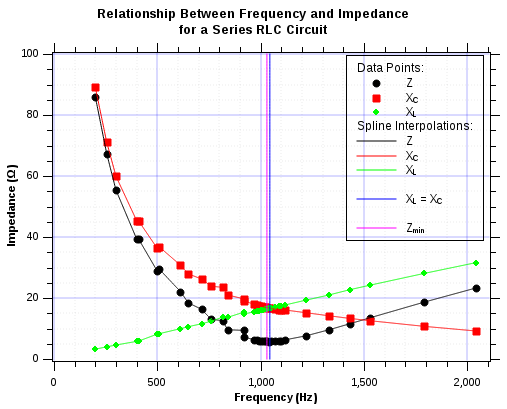
\includegraphics[width=\linewidth]{./Part2.png}
	\caption{Plot of $X_L, X_C, $ and $Z$ vs. $f$. The resonant frequency is determined from the intersection of the $X_C$ and $X_L$ curves, and the resistance of the circuit is given at the minimum of the $Z$ curve.}
	\label{fig:xf_graph1}
	\end{center}
	\par\end{centering}
\end{figure}

From the plotted data, we have
\hfill\underline{$Z_{\text{min}} = R_{\text{meas}} = 5.72 \Omega$}

\hfill\underline{$f_{\text{res,meas}} = 1044$ Hz} \\

\textit{Why is $R$ (meas) not the same value of the resistor used in the circuit?}

This indicates that there was resistance in the circuit that was unaccounted for. Possible sources for this resistance are the inductor coils, the internal resistance of the power supply, and erosion or damage to the terminal contacts.
\hrulefill

\subsection{Current vs. Frequency}

%$(V*2*pi*x) * ((R*2*pi*x)^2 + L^2*((2*pi*x)^2 - O^2)^2)^(-1/2)$

The data points were fitted to the function
\begin{equation}
	I_{\text{rms}}(\omega)
	= \frac
	{V_{\text{rms}}\omega}
	{\sqrt{(R\omega)^2 +L^2(\omega^2-\omega_0^2)^2}}
\end{equation}

\begin{figure}[H]
	\begin{centering}
	\begin{center}
	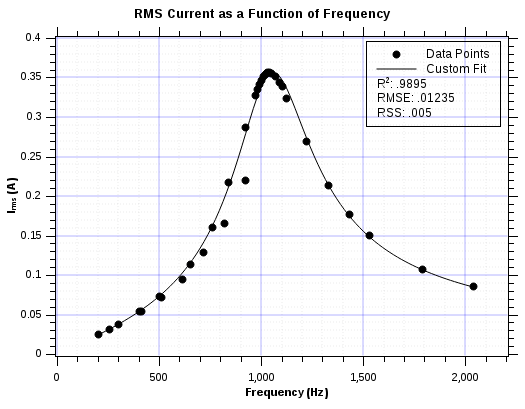
\includegraphics[width=\linewidth]{./Part3.png}
	\caption{Plot of $I_{\text{rms}}$ vs. $f$. $V_{\text{rms}}$ and $L_{\text{avg}}$ were used as constants, while $R$ and $\omega_0$ were left as fitting parameters.}
	\label{fig:IvsFreq}
	\end{center}
	\par\end{centering}
\end{figure}

From the custom fit described above, the values obtained from the fitting parameters were:

\hfill\underline{$R_{\text{fit}} = 5.80 \pm .06 \Omega$}

\hfill\underline{$f_{\text{res, fit}} = 1059 \pm 5$ Hz}


\hrulefill

\subsection{Difference between measured and fitted values}

\textit{What is the percent difference between $R$ (measured) and $R$ (fit)? Is $R$ (measured) within the uncertainty of $R$ (fit)?}

\hfill\underline{Percent Difference: $0.87\%$}

The uncertainty in $R$ (fit) was $.06\Omega$ -- however, the values differed by $.08\Omega$. While the two values are generally in good agreement, there are slight errors introduced in the interpolation used to find $Z$ (min) on the graph, as well as a certain amount of random error introduced by transient voltage fluctuations when the circuit is near resonance. However, both values are relatively consistent with each other, so we deduce that this value more accurately represents the actual resistance present in the circuit than the value measured with the ohmmeter.

\hrulefill

\subsection{Theoretical Resonant Frequency}
The resonant frequency, calculated from the mean values of $L$ and $C$ from step 1 is given by
\begin{align}
	f_{\text{res,theor}} &= \frac{1}{2\pi\sqrt{L_{\text{avg}} C_{\text{avg}}}}.
\end{align}

So the theoretical resonant frequency is:

\hfill\underline{$f_{0(\text{theor})} = 1064$ Hz} \\

Comparing this to the values determined in Steps 2 and 3 above, we have

\hfill\underline{\% Difference, Step 2: $1.9\%$}

\hfill\underline{\% Difference, Step 3: $0.47\%$}

\hrulefill

\subsection{Voltage vs Frequency}

\begin{figure}[h!]
	\begin{centering}
	\begin{center}
	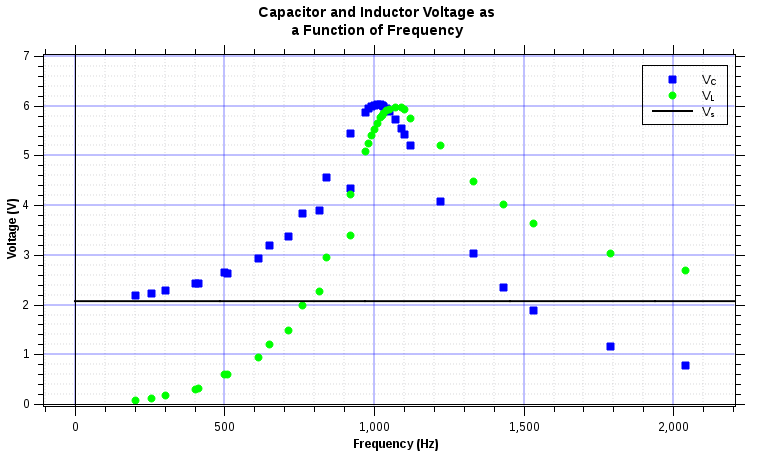
\includegraphics[width=\linewidth]{./Part6.png}
	\caption{Plot of $V_L$ and $V_C$ vs $f$, extrapolated to zero frequency.}
	\label{fig:VvsFreq}
	\end{center}
	\par\end{centering}
\end{figure}

\textit{What does this graph tell you?}

Several things are apparent from the graph -- the most immediate characteristic of the series RLC circuit is that in the limit of low frequencies, the voltage on the capacitor $V_C$ approaches the source voltage. This agrees with our theoretical understanding of the behavior of a capacitor, which would tend to act as a short circuit at low frequencies. This effect can also be recovered by considering the equation for the impedance of the capacitor, $X_C = 1/2\pi f C$, which predicts that the impedance approaches infinity as the frequency approaches zero. An infinite impedance is effectively a short, necessarily implying that no current will flow and the capacitor will be forced to remain at the potential difference of the source. This is reflected in the graph, as the low-frequency limit of the capacitor voltage approaches the source voltage.

A symmetric but opposite is observed in the inductor, for which the voltage $V_L$ approaches zero in the low-frequency limit. From the impedance equation $X_L = 2\pi f L$, we see that in this limit, the impedance approaches zero -- effectively creating an shunt in the circuit. This causes the inductor to behave like a wire, which agrees with our theoretical model of inductance.

In the limit of high frequencies, the behavior of the inductor and the capacitor switch roles. Both voltages peak symmetrically about the resonant frequency, and the capacitor voltage then approaches zero while the inductor voltage approaches the source voltage. These effects can be seen by considering the limit as $f$ approaches infinity in the previously mentioned inductance equations, and noting that the capacitor's impedance tends to zero while the inductor's impedance tends to infinity. This leads to the capacitor now behaving like a wire, and the inductor like a shunt, which again agrees with our theoretical model of impedance.

The last important characteristic of this graph shows that the maximum voltage is delivered at the resonant frequency. This occurs midway between the maximums the two individual curves, and represents the point at which maximum power is delivered.

\hrulefill

\subsection{Phase Angle vs. Frequency}

\begin{figure}[H]
	\begin{centering}
	\begin{center}
	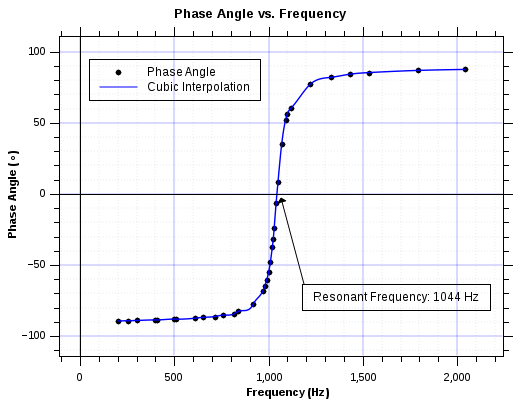
\includegraphics[width=\linewidth]{./Part7.png}
	\caption{Plot of phase angle ($360^{\circ}f\Delta t$) vs. $f$. The y-intercepts represents the frequency at which the current and the voltage are in phase, and corresponds to the circuit's resonant frequency. }
	\label{fig:PhasevsFreq}
	\end{center}
	\par\end{centering}
\end{figure}

\textit{Does this curve agree with theory? Explain.}

The curve agrees with theory in several ways. The most noticeable factor is that the phase angle is equal to zero at exactly the same value found in previous fits. This agrees with the notion that having the current and voltage in phase results in circuit resonance. The graph also shows that the phase angle is negative below resonance, and positive above resonance, approaching $\pm 90^{\circ}$ as $f$ approaches $\infty$ and $0$ respectively. From the expression
\begin{align}
	\phi = \frac{X_L-X_C}{R} = \frac{\omega L - \frac{1}{\omega C}}{R},
\end{align}
we see that as the frequency approaches infinity, $X_C$ goes to zero and we expect the circuit to be primarily inductive. In this case, we would expect the voltage to lead the current, which is reflected in the positive phase angle above resonance.

As the frequency approaches zero, $X_L$ goes to zero, and we would expect the circuit to be more capacitive. This would lead to the current leading the voltage -- or in other words, the voltage lagging the current. This is also reflected in the negative phase angles below resonance.

\hrulefill

\subsection{Power vs. Frequency}

\begin{figure}[H]
	\begin{centering}
	\begin{center}
	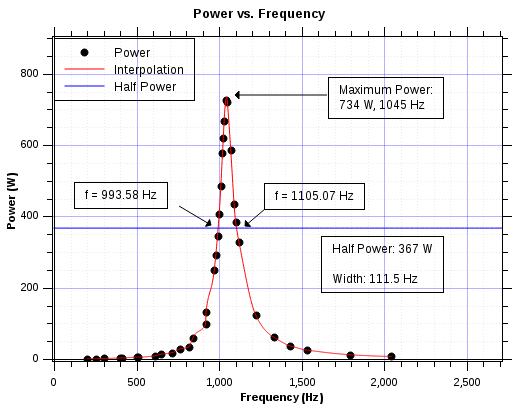
\includegraphics[width=\linewidth]{./Part8.png}
	\caption{Plot of $P$ vs $f$, used to determine the full-width at half-max in order to calculate $Q$.}
	\label{fig:PowervsFreq}
	\end{center}
	\par\end{centering}
\end{figure}

Bandwidth: \hfill\underline{$\Delta f$ = 111.5 Hz}

\hrulefill

\subsection{Quality Factor}
The calculated quality factor is given by
\begin{equation}
	Q_{\text{calc}} = \frac{f_{\text{max, meas}}}{\Delta f}
\end{equation}

The theoretical Quality factor is given by
\begin{equation}
	Q = \frac{\omega_0 L}{R_{\text{meas}}},
\end{equation}
where $\omega_0$ is given by $2\pi f_{\text{res,meas}}$ from Step 2 and $L$ is $L_{\text{avg}}$ from Step 1.

And the uncertainty in $Q$ is given by
\begin{equation}
	\sqrt{(\frac{\partial Q}{\partial f})^2(\delta f)^2 + (\frac{\partial Q}{\partial \Delta f})^2(\delta \Delta f)^2}
\end{equation}

Assuming an uncertainty of 1 Hz in both $f$ and $\Delta f$, we have: \\


\hfill Calculated Quality Factor: \underline{$Q_{\text{calc}} = 2.919\pm .009$}

\hfill Theoretical Quality Factor: \underline{$Q = 2.904$}

\hfill Percent Difference: \underline{0.52\%}

\hrulefill

%\appendices{}
%\bibliographystyle{plain}
%\bibliography{physbib}

\end{document}